ONOS\footnote{Open Network Operating System} est un contrôleur SDN open source récent (début en décembre 2014, la fondation Linux arrive en octobre 2015 dans le projet), écrit en java, déployable avec Maven et utilisant apache-karaf comme conteneur OSGi (qui fournit entre autre l’interface utilisateur permettant l’interaction avec le contrôleur).
La version actuelle est Goldeneye (juin 2016) (1.6), la prochaine Hummingbird.
C'est un projet basé sur la technique \footnote{\url{http://onosproject.org/governance/}} : \begin{quote}
goal is to « provide an environment that thrives on technical meritocracy. Merit is based on technical contribution, not on financial contribution. »
\end{quote}

Le contrôleur est architecturé de la manière suivante :
\begin{figure}[h]
  	\centering
  	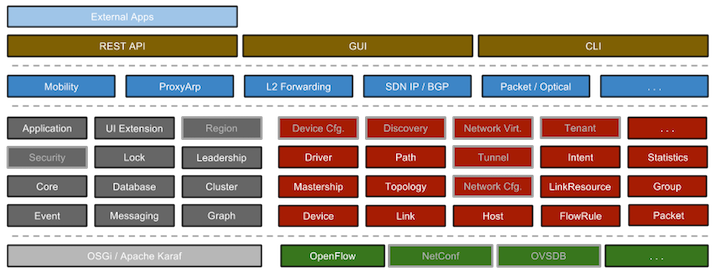
\includegraphics[width=1\textwidth]{ONOS_archi.png}
  	\caption{Architecture logicielle d'ONOS (schéma extrait du site officiel)}
\end{figure}

\begin{list}{$\Asteriscus$}{}

\item Au Sud : une API (southbound) gérant plusieurs protocoles (dont Openflow (toutes les versions jusqu’à la version 1.5, la version 1.6 étant en cours de prise en charge)). C’est la partie d’ONOS qui se charge de la communication avec les switchs. Il est ainsi possible de prendre en charge de nouveaux protocoles ou de nouveaux drivers.

\item Sur le côté : un protocole d’échange entre contrôleurs. Cela permet un contrôle partagé du réseau. Pour cela, des informations sur la topologie de celui-ci doivent être échangées entre contrôleurs. Le protocole en question n'est pas standardisé.

\item Au Nord : une API (northbound) permettant d’écrire des applications utilisant les ressources offertes par le contrôleur. Si le secure mode est activé (nous reviendrons plus en détail sur cela ultérieurement), l’ensemble des méthodes utilisables est restreint. 

\item Au Nord encore : une interface utilisateur fournie par Karaf et composée de 3 parties: une API REST accessible sur le port 8181 (configurable), une interface web (permettant de visualiser l’état du réseau, les applications lancées ...) accessible sur ce même port, et une CLI accessible en SSH sur le port 8101 (ou bien directement sur le contrôleur, là encore tout est configurable).

\end{list}